\documentclass{statsmsc}
\usepackage{float}
\usepackage{hyperref}
\usepackage[utf8]{inputenc}
\usepackage{graphicx}
\usepackage{caption}
\usepackage{subcaption}
\usepackage{algpseudocode}
\usepackage{algorithm}
\usepackage{mathtools}
\usepackage{amsmath,amssymb}
\usepackage{nccmath}
\usepackage{siunitx}
\usepackage{listings}
\usepackage{physics}
\usepackage{tikz}
\usepackage[outline]{contour} % glow around text
\usepackage{bbm}
\usepackage[most]{tcolorbox}
\newcommand{\e}[1]{{\mathbb E}\left[ #1 \right]}
\definecolor{block-gray}{gray}{0.90}
\newtcolorbox{code}{colback=block-gray,grow to right by=-1mm,grow to left by=-1mm,boxrule=0pt,boxsep=0pt,breakable}
\lstset{
  basicstyle=\ttfamily,
  columns=fullflexible,
  frame=single,
  breaklines=true,
  postbreak=\mbox{\textcolor{red}{$\hookrightarrow$}\space},
}
\usetikzlibrary{patterns,snakes}
\usetikzlibrary{arrows.meta} % for arrow size
\contourlength{0.4pt}

\colorlet{xcol}{blue!70!black}
\colorlet{darkblue}{blue!40!black}
\colorlet{myred}{red!65!black}
\tikzstyle{mydashed}=[xcol,dashed,line width=0.25,dash pattern=on 2.2pt off 2.2pt]
\tikzstyle{axis}=[->,thick] %line width=0.6
\tikzstyle{ell}=[{Latex[length=3.3,width=2.2]}-{Latex[length=3.3,width=2.2]},line width=0.3]
\tikzstyle{dx}=[-{Latex[length=3.3,width=2.2]},darkblue,line width=0.3]
\tikzstyle{ground}=[preaction={fill,top color=black!10,bottom color=black!5,shading angle=20},
                    fill,pattern=north east lines,draw=none,minimum width=0.3,minimum height=0.6]
\tikzstyle{mass}=[line width=0.6,red!30!black,fill=red!40!black!10,rounded corners=1,
                  top color=red!40!black!20,bottom color=red!40!black!10,shading angle=20]
\tikzstyle{spring}=[line width=0.8,blue!7!black!80,snake=coil,segment amplitude=5,segment length=5,line cap=round]
\tikzset{>=latex} % for LaTeX arrow head
\tikzstyle{force}=[->,myred,very thick,line cap=round]
\def\tick#1#2{\draw[thick] (#1)++(#2:0.1) --++ (#2-180:0.2)}
\newsavebox{\overlongequation}
\newenvironment{CentreLongEquation}
 {\begin{displaymath}\begin{lrbox}{\overlongequation}$\displaystyle}
 {$\end{lrbox}\makebox[0pt]{\usebox{\overlongequation}}\end{displaymath}}


\title{Learning Invariances in Dynamical System}
\author{Cheng-Cheng Lao}
\CID{01353756}
\supervisor{Dr. Andrew Duncan and Dr. Mark van der Wilk}
\date{\today}
%For today's date, use:
%\date{\today}
\logoimg{}


% THIS IS WHERE NEW COMMANDS CAN BE DEFINED
% commands below only used in the proof; otherwise can be deleted
\newcommand{\consta}{a}
\newcommand{\X}{X}
\newcommand{\EE}[1]{ \mathrm{E} [ #1 ] }
\newcommand{\inparenth}[1]{\left( #1 \right)}

\begin{document}

% Generates the Title Page
\maketitle


% Generates plagiarism declaration
\declarationname{Cheng-Cheng Lao}
\declarationdate{\today}
\declaration 


\begin{abstract}
    ABSTRACT GOES HERE
\end{abstract}

\begin{acknowledgements}
    ANY ACKNOWLEDGEMENTS GO HERE
\end{acknowledgements}

% add glossary?

% VERY IMPORTANT
% This command switches from Roman to Arabic numbering for main part of thesis
\mainmatter


\chapter{Introduction}

The introduction section goes here\footnote{Tip: write this section last.}.

\chapter{Background}
Here we will cover the background knowledge required to understand the remaining thesis, including theortical foundation of Gaussian Process, dynamical systems and invariances. 

Background chapter.

\section{Gaussian Process}
Gaussian Process (GP)


A subsubsection.
\section{Dynamical Systems}
A dynamical system is simply a system that evolves with time under some kind of rules.
\section{Invariances}
Invariances are functions of the states that describe a dynamical system, and is unchanged throughout the evolution of the system over time. 
An example would be from the field of physics, the conservation of energy, which will be unchanged throught out the trajectories of the system.
\section{GPflow}

\section{Related Work}
\subsection{Physics Informed Machine Learning}
\subsection{Learning Invariance using Marginal Likelihood}
\subsection{Symmetry and Invariances}
\subsection{Symbolic approach}



\chapter{Invariance Kernel}
In this chapter we will start with general theoretical construction of invariance kernel given the knowlwedge of the invariance of the system.
We will then apply the construction to various systems, namely linear and nonlinear system in both one and two dimensions.
\section{General Construction}
If we are given a dynamical system of dimension d with variables $\mathbf{q}, \mathbf{p}$, where $\mathbf{q} = (q_1, q_2,\dots,q_d)$ is the vector of positional coordinates, and $\mathbf{p}=(p_1, p_2, \dots, p_d)$ is the vector of velocity coordinates of the states of the dynamical system.
We are interested to predict the future trajectories of the state of the system.
Therefore, we would like to know the time derivative of these coordinates so we can update them according to Euler's integrator. 
These time derivatives are referred to as the dynamics of a dynamical system, which governs the evolution of the dynamical system, and is a function of the coordinates $\mathbf{q}$ and $\mathbf{p}$ 
For our systems, we will denote the dynamics of $\mathbf{p}$ as $\frac{d\mathbf{p}}{dt}=\mathbf{a}(\mathbf{q}, \mathbf{p})$, and that of $\mathbf{q}$ as $\frac{d\mathbf{q}}{dt}=\mathbf{v}(\mathbf{q}, \mathbf{p})$.
Once we have the dynamics, we can integrate up to obtain the future trajectories. 
Notation wise, we will collect the two dynamics term and call them $$\mathbf{f(\mathbf{q}, \mathbf{p})}=\begin{pmatrix}
    \mathbf{a(\mathbf{q}, \mathbf{p})}\\\mathbf{v(\mathbf{q}, \mathbf{p})}
\end{pmatrix}$$
For simplicity of notation, the dependence on $\mathbf{q}, \mathbf{p}$ is now implicit. 
We will put independent GP prior on $\mathbf{a}$ and $\mathbf{v}$ since there are no reason we should assume they are correlated. 
For the choice of kernel, we chose the standard smooth kernel, the squared exponential kernel, or RBF, and we denote this kernel to be $K_{RBF}$. 
We will also denote any set of coordinates of length $n$ and dimension $d$ as $$X=\begin{pmatrix}
    q_{11}& q_{21} &\dots& q_{d1} & p_{11} & p_{21} & \dots & p_{d1} \\
    q_{12}& q_{22} &\dots& q_{d2} & p_{12} & p_{22} & \dots & p_{d2} \\
    \vdots &\vdots &\ddots &\vdots &\vdots &\vdots &\ddots &\vdots \\
    q_{1n}& q_{2n} &\dots& q_{dn} & p_{1n} & p_{2n} & \dots & p_{dn} \\
\end{pmatrix}=\begin{pmatrix}
    \mathbf{x}_1\\\mathbf{x}_2\\\vdots\\\mathbf{x}_n
\end{pmatrix}.$$
Without loss of generality, we will choose to stack the dynamics vertically in $\mathbf{f}$; for example in a d dimensional system, we have $$\mathbf{f}(X)=\begin{pmatrix}
    a_1(\mathbf{x}_1)\\
    \vdots\\
    a_1(\mathbf{x}_n)\\
    \vdots\\
    a_d(\mathbf{x}_1)\\
    \vdots\\
    a_d(\mathbf{x}_n)\\
    v_1(\mathbf{x}_1)\\
    \vdots\\
    v_1(\mathbf{x}_n)\\
    \vdots\\
    v_d(\mathbf{x}_1)\\
    \vdots\\
    v_d(\mathbf{x}_n)\\
\end{pmatrix}$$
For our naive independent RBF GP prior, we have 
\begin{CentreLongEquation}
$$
K=\mathrm{Cov}(\mathbf{f}(X), \mathbf{f}(X'))=\begin{pmatrix}
    K_{RBF,a_1}(X,X') & \dots  & \dots          & \dots         & 0\\
    \vdots        & \ddots & \dots          & \ddots        & \vdots\\
    0             & \dots  & K_{RBF,a_d}(X,X')  & \dots         & 0 \\
    \vdots        & \ddots & \vdots         & K_{RBF,v_1}(X,X') & \vdots \\
    0             & \dots  & 0              & \dots         & K_{RBF,v_d}(X,X')\\
\end{pmatrix},
$$
\end{CentreLongEquation}

with all the off diagonal terms being zero block matrix because of the independence prior assumption.
This naive kernel will be our baseline to be compared to throughout the whole project.
Now we can start considering the invariance. 
If we assume the invariance is true throughout the input space $\mathbb{R}^{2d}$, then we can condition the GP on the a grid of points, which we referred to invariance points, $X_L$, and assume it has length $\ell$, and we will call the invariance constraints $L$.
The form of $L$ will depend on the system as well as $X_L$, and examples will be described in the following sections.
Since the invariance function will always be a linear function on the dynamics, if we apply this linear transformation $L$ on $\mathbf{f}(X_L)$, $L(\mathbf{f}(X_L))$ will again be a GP with a transformed kernel.
Therefore, we have 
$$\begin{pmatrix}
\mathbf{f}(X)\\L[\mathbf{f}(X_L)]
\end{pmatrix}
\sim\mathcal{N}
\left(\begin{pmatrix}0_{2nd}\\0_{\ell}\end{pmatrix}, \begin{pmatrix}
    K & LK \\
    KL^T & LKL^T\\
\end{pmatrix}\right)
$$

\section{1D System}
\subsection{Linear}
We will first examine one of the most simple dynamical system, an 1D simple harmonic motion (SHM). 
An example would be a mass spring system as shown in figure with mass $m$ and spring constant $k$. 

% HORIZONTAL spring - axis, rest position
\begin{figure}[H]
    \centering
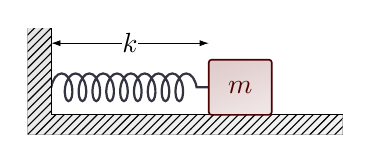
\begin{tikzpicture}
  \def\H{1.1}  % wall height
  \def\T{0.3}  % wall thickness
  \def\W{3.7}  % ground length
  \def\D{0.25} % ground depth
  \def\h{0.7}  % mass height
  \def\w{0.8}  % mass width
  \def\x{2.0}  % mass x position
  \def\y{1.22*\H} % x axis y position
  
  % AXIS
  \draw[ell] (0,1.3*\h) --++ (\x,0) node[midway,fill=white,inner sep=0] {$k$};
  
  % SPRING & MASS
  \draw[spring] (0,\h/2) --++ (\x,0);
  \draw[ground] (0,0) |-++ (-\T,\H) |-++ (\T+\W,-\H-\D) -- (\W,0) -- cycle;
  \draw (0,\H) -- (0,0) -- (\W,0);
  \draw[mass] (\x,0) rectangle++ (\w,\h) node[midway] {$m$};
  
\end{tikzpicture}
\end{figure}

The defining equation is $$m\frac{d^2q}{dt^2}=-kq$$, where $q$ is the displacement.
And the analytical solution would be of the form $q=A\sin(\omega_0t+\phi),$ where $\omega=\frac{k}{m}$ and $A, \phi$ depends on the initial condition, which dictates the amplitude and phase of the motion. 
For this case, we have 
$$
\mathbf{f}(X)=\begin{pmatrix}
    \mathbf{a}(X)\\
    \mathbf{v}(X)\\
\end{pmatrix}
$$
We also have the energy, $E=\frac{mp^2}{2}+\frac{kq^2}{2},$
Therefore, to obtain our invariance $L$, we use the conservation of energy $\frac{dE}{dt}=0$ so we finally have $$L(a, v)=mpa+kqv=0$$
While $L$ is not able to be into a matrix form, it is an linear operator as shown below. 
If we have $$X_L=\begin{pmatrix}
    q_{L,1} & p_{L,1}\\
    \vdots & \vdots \\
    q_{L,\ell} & p_{L,\ell}\\
\end{pmatrix}=\begin{pmatrix}
    \vdots & \vdots\\
    q_L & p_L\\
    \vdots & \vdots\\
\end{pmatrix}=\begin{pmatrix}
    \mathbf{x}_{L,1}\\
    \vdots\\
    \mathbf{x}_{L,\ell}\\
\end{pmatrix},$$
then we have 
$$
L([\mathbf{f}(X_L)]) = \begin{pmatrix}
   mp_{L,1}a(q_{L,1},p_{L,1}) + kq_{L,1}v(q_{L,1},p_{L,1})\\ 
   \vdots \\
   mp_{L,\ell}a(q_{L,\ell},p_{L,\ell}) + kq_{L,\ell}v(q_{L,\ell},p_{L,\ell})\\ 
\end{pmatrix}.
$$
Combine with original GP prior assumption, we will have 
$$
\begin{pmatrix}
    \mathbf{f}(X)\\
    L([\mathbf{f}(X_L)])\\
\end{pmatrix}
\sim\mathcal{N}
\left(\begin{pmatrix}
    0_{2n}\\0_{\ell}
\end{pmatrix},\begin{pmatrix}
   A & B \\
   C & D\\ 
\end{pmatrix}\right),
$$
where
$$
A=K(X,X), B=\begin{pmatrix}
    K_{RBF,a} \\ K_{RBF,v} \\
\end{pmatrix}\odot \begin{pmatrix}
    mP_L \\ kQ_L
\end{pmatrix}, C=B^T, D=K_{RBF,a}\odot m^2(p_L\otimes p_L) + K_{RBF,v}\odot k^2(q_L\otimes q_L),
$$
where $\odot$ is the element wise product and $\otimes$ is the Kronecker product so that 
$$
P_L=\begin{pmatrix}
  p_{L,1}  & \dots & p_{L,\ell}  \\
  \vdots & \text{repeats n rows} &  \vdots\\
  p_{L,1}  & \dots & p_{L,\ell}  \\
\end{pmatrix},
Q_L=\begin{pmatrix}
  q_{L,1}  & \dots & q_{L,\ell}  \\
  \vdots & \text{reqeats n rows} &  \vdots\\
  q_{L,1}  & \dots & q_{L,\ell}  \\
\end{pmatrix}
$$
and we have 
$$
p_L\otimes p_L=\begin{pmatrix}
  p_{L,1}^2 & p_{L,1}p_{L,2} & \dots & p_{L,1}p_{L,\ell} \\
  \vdots & \vdots & \vdots & \vdots \\
  p_{L,\ell}p_{L,1} & p_{L,\ell}p_{L,2} & \dots & p_{L,\ell}^2 \\
\end{pmatrix},
q_L\otimes q_L=\begin{pmatrix}
  q_{L,1}^2 & q_{L,1}q_{L,2} & \dots & q_{L,1}q_{L,\ell} \\
  \vdots & \vdots & \vdots & \vdots \\
  q_{L,\ell}q_{L,1} & q_{L,\ell}q_{L,2} & \dots & q_{L,\ell}^2 \\
\end{pmatrix},
$$ 
These matrices can be obtained if we try to compute the covariance manually. 
For $B$, we wish to calculate 

\begin{align*}
B_{ij} &= \mathrm{Cov}(\mathbf{f}(X), L[\mathbf{f}(X_L)])_{ij} \\
       &= \mathrm{Cov}(\mathbf{f}(X)_i, L\mathbf{f}(X_L)_j) \\ 
       &= \begin{cases}
        \mathrm{Cov}(a(q_i, p_i), mp_{L,j}a(q_{L,j},p_{L,j}) + kq_{L,j}v(q_{L,j},p_{L,j})) & i\le n \\ 
        \mathrm{Cov}(v(q_i, p_i), mp_{L,j}a(q_{L,j},p_{L,j}) + kq_{L,j}v(q_{L,j},p_{L,j})) & i>n \\ 
       \end{cases} \\
       &= \begin{cases}
        K_{RBF,a}(\mathbf{x}_i, \mathbf{x}_{L,j}) mp_{L,j} & i\le n \\ 
        K_{RBF,v}(\mathbf{x}_i, \mathbf{x}_{L,j}) kq_{L,j} & i>n \\ 
       \end{cases}, \\
\end{align*}
and hence we have the form above. 
For $D$, we have
\begin{align*}
D_{ij} &= \mathrm{Cov}(L[\mathbf{f}(X_L)], L[\mathbf{f}(X_L)])_{ij} \\
       &= \mathrm{Cov}(mp_{L,i}a(q_{L,i},p_{L,i}) + kq_{L,i}v(q_{L,i},p_{L,i}), mp_{L,i}a(q_{L,i},p_{L,i}) + kq_{L,i}v(q_{L,i},p_{L,i})) \\
       &= m^2p_{L,i}p_{L,j}K_{RBF,a}(\mathbf{x}_{L,i},\mathbf{x}_{L,j}) + k^2q_{L,i}q_{L,j}K_{RBF,v}(\mathbf{x}_{L,i},\mathbf{x}_{L,j})
\end{align*}
using the bilnear property of the covariance operator and the fact that $v$ and $a$ are independent.
Since we assume invariance on these invariance points, we will condition on $L([\mathbf{f}(X_L)])=0.$
Now we can simply use the Gaussian conditional formula to obtain the Schur Complement
$$
\mathbf{f}(X)|L[\mathbf{f}(X_L)]=0\sim\mathcal{N}(0_{2n},A-BD^{-1}C),
$$
we will then call the covariance part our Invariance Kernel for 1D SHM, $K_L$.
\subsection{Non Linear}
The story is pretty much the same for nonlinear system, it is just the fitting would be expected to be more difficult.
A simple nonlinear system in every day life is a simple pendulum as shown in figure below.
The governing equation is 
$$
\frac{d^2q}{dt^2}=-\frac{g}{\ell}\sin q, 
$$
where $q$ is the angle of displacement this time. 
The nonlinear dynamics bit occurs because of the sine term, which will complicate things slightly. 
However, since $\sin x \approx x$ at small angle, this system is approximately linear under small displacement. 
There is no analytical solution to this nonlinear problem.
This time we have energy, $E=\frac{m\ell^2p^2}{2}+mg\ell(1-\cos q)$, and by setting the time derivative to 0, we have 
$$L(a, v)=\frac{dE}{dt}=m\ell^2pa+mg\ell(\sin q)v=0.$$
If we cancel out the common term $m\ell$ since their product cannot be zero, we have $$L(a,v)=\ell pa+g(\sin q)v=0$$
Most of the terms are unchanged from the linear case. 
However, this time, 
$$
B=\begin{pmatrix}
    K_{RBF,a} \\ K_{RBF,v} \\
\end{pmatrix}\odot \begin{pmatrix}
    \ell P_L \\ g\sin(Q_L)
\end{pmatrix}, D=K_{RBF,a}\odot \ell^2(p_L\otimes p_L) + K_{RBF,v}\odot g^2(\sin(q_L)\otimes \sin(q_L)),
$$
where 
$$
\sin(Q_L) = g\begin{pmatrix}
  \sin(q_{L,1})  & \dots & \sin(q_{L,\ell})  \\
  \vdots & \text{reqeats n rows} &  \vdots\\
  \sin(q_{L,1})  & \dots & \sin(q_{L,\ell})  \\
\end{pmatrix},
$$
$$
\sin(q_L)\otimes \sin(q_L)=\begin{pmatrix}
  \sin(q_{L,1})^2 & \sin(q_{L,1})\sin(q_{L,2}) & \dots & \sin(q_{L,1})\sin(q_{L,\ell}) \\
  \vdots & \vdots & \vdots & \vdots \\
  \sin(q_{L,\ell})\sin(q_{L,1}) & \sin(q_{L,\ell})\sin(q_{L,2}) & \dots & \sin(q_{L,\ell})^2 \\
\end{pmatrix},
$$
derived in almost exactly the same way as the linear case. 
\section{Damped System}
Before we have considered a perfect system, i.e. a system in an ideal world without frictions and the conservation of energy is perfectly obeyed such that $L=0$ exactly.
However, in a real world system, there will be dissipation where energy is lost in the form of heat etc.  
Therefore, to model that, we need to allow "approximate" invariance, such that the invariance $L$ is noisy and not always equal to zero. 
To do so, it is similar in spirit to when we add noise to the underlying GP to represent noise signal, where we have $K+\sigma_n^2 \mathbb{I}$.
Here, since the white noise is uncorrelated, the only place the noise will enter is $D$, so we simply have to add a noise term to $D$ and replace all $D$ with $\tilde{D}=D+\epsilon \mathbb{I}$, where $\epsilon$ is a parameter to be learnt. 
\section{2D System}
A 2D system is not that different from an 1D system. The major difference being there are two more extra variables. 
We again look at two simple examples, a linear 2D SHM, and a nonlinear double pendulum.
\subsection{Linear}
A simple extension to 1D SHM to 2D is just allowing the spring to be at an angle so that the system is now in a 2D space.
Again, the equations are simple that we have two equations for the two coordinates.
$$
\begin{cases}
    \frac{d^2{q_1}}{dt^2} = -\frac{k}{m}q_1\\
    \frac{d^2{q_2}}{dt^2} = -\frac{k}{m}q_2\\
\end{cases}
$$
The analytical solution is exactly the same, but now there are two of them with differing amplitudes and phases depending on the initial condition. 
And now we have $$\mathbf{f}(X)=\begin{pmatrix}
    \mathbf{a_1}(X)\\
    \mathbf{a_2}(X)\\
    \mathbf{v_1}(X)\\
    \mathbf{v_2}(X)\\
\end{pmatrix},$$
where $\mathbf{a_1}$ and $\mathbf{a_2}$ are the dynamics or time derivative for $\mathbf{p_1}$ and $\mathbf{p_2}$ respectively; similarly $\mathbf{v_1}$ and $\mathbf{v_2}$ are the time derivative of $\mathbf{q_1}$ and $\mathbf{q_2}$.
In this system, the energy is the sum of energy in the two directions so $E=\frac{m(p_1^2+p_2^2)}{2}+\frac{k(q_1^2+q_2^2)}{2}$ and so the invariance $L(a_1, a_2, v_1, v_2)=mp_1a_1+mp_2a_2+kq_1v_1+kq_2v_2=0.$
Now our naive baseline GP has the kernel
$$
K(X,X')=\begin{pmatrix}
K_{RBF,a_1}(X,X') & 0 & 0 & 0 \\
0 & K_{RBF,a_2}(X,X') & 0 & 0 \\
0 & 0 & K_{RBF,v_1}(X,X') & 0 \\
0 & 0 & 0 & K_{RBF,v_2}(X,X') \\
\end{pmatrix}.
$$
We will then have the joint distribution of
$$
\begin{pmatrix}
    \mathbf{f}(X)\\L[\mathbf{f}(X_L)]\\
\end{pmatrix}
\sim\mathcal{N}
\left(
\begin{pmatrix}
    0_{4n} \\ 0_{\ell}
\end{pmatrix},
\begin{pmatrix}
    A & B \\
    C & D\\
\end{pmatrix}
\right),
$$
with 

$$
A=K(X, X'), 
B=\begin{pmatrix}
    K_{RBF, a_1}\\
    K_{RBF, a_2}\\
    K_{RBF, v_1}\\
    K_{RBF, v_2}\\
\end{pmatrix}\odot
\begin{pmatrix}
mP_{1L}  \\
mP_{2L}  \\
kQ_{1L}  \\
kQ_{2L}  \\
\end{pmatrix},
C=B^T 
$$

\begin{gather*}
D=K_{RBF,a_1}m^2\odot(p_{1L}\otimes p_{1L}) + K_{RBF,a_2}m^2\odot(p_{2L}\otimes p_{2L})\\+K_{RBF,v_1}k^2\odot(q_{1L}\otimes q_{1L})+K_{RBF,v_2}k^2\odot(q_{2L}\otimes p_{2L})
\end{gather*}

where the terms are defined the exact same way as before, but now with respect to different coordinates, and the derivation are also the same.
We will then again take the Schur Complement.
\subsection{Non Linear}
Now we will to introduce double pendulum, which is a fairly nonlinear system and quite complicated. 
It has two mass blobs $m_1$ and $m_2$ as well as two lengths for the pendlum stem $\ell_1$ and $\ell_2$.
The defining equations are as follows:
$$
\begin{cases}
\frac{d^2q_1}{dt^2}=\frac{-g\left(2 m_{1}+m_{2}\right) \sin q_1-m_{2} g \sin \left(q_1-2 q_2\right)-2 \sin \left(q_1-q_2\right) m_{2}\left(p_2^{2} l_{2}+p_1^{2} l_{1} \cos \left(q_1-q_2\right)\right)}{l_{1}\left(2 m_{1}+m_{2}-m_{2} \cos \left(2 q_1-2 q_2\right)\right)} \\
\frac{d^2q_2}{dt^2}=\frac{2 \sin \left(q_1-q_2\right)\left(p_1^{2} l_{1}\left(m_{1}+m_{2}\right)+g\left(m_{1}+m_{2}\right) \cos q_1+p_2{ }^{2} l_{2} m_{2} \cos \left(q_1-q_2\right)\right)}{l_{2}\left(2 m_{1}+m_{2}-m_{2} \cos \left(2 q_1-2 q_2\right)\right)}
\end{cases}
$$
As we can see, it is very complicated in term of the form.
We also have form of energy 
$$
E = -(m_1+m_2)gl_1\cos q_1-m_2gl_2\cos q_2+ \frac{m_1l^2_1p_1^2}{2}+\frac{m_2}{2}(l^2_1p_1^2+l^2_2p_2^2+2l_1l_2p_1p_2\cos(q_1-q_2))
$$
While the form is more complicated, the underlying principle to construct the invariance kernel. 
We again differentiate with respect to time and set it to zero to obtain the invariance equation to obtain 
\begin{gather*}
L(a_1, a_2, v_1, v_2)=\frac{dE}{dt} = (m_1+m_2)gl_1\sin\theta_1v_1+m_2gl_2\sin\theta_2v_2+m_1l_1^2\dot{\theta}_1a_1+\\m_2(l_1^2\dot{\theta}_1a_1+l_2^2\dot{\theta}_2a_2+l_1l_2(\dot{\theta}_2\cos(\theta_1-\theta_2)a_1+\dot{\theta}_1\cos(\theta_1-\theta_2)a_2-\dot{\theta_1}\dot{\theta_2}\sin(\theta_1-\theta_2)(v_1-v_2)))=0
\end{gather*}
The form of the invariance matrix is too cubersome to write down, but the derivation is as straightforward as before. 

\section{Local Invariance}
Conditioning on a grid of invariance points is simply not scalable in high dimensions. 
If we have an invariance density of 1 in a $\pm 5$ range for 2D SHM, then we will have 10000 points. 
We will easily run out of memory and also taking the matrix inverse are very difficult and time consuming.
As a result, to make the approach scalable to 2D space, we will use the idea of local invariance. 
Which is to take samples in the local region around training and testing points and condition on these points.
Hopefully that will constraint our results enough. 


\chapter{Learning Invariance}
Previously, we have assumed the knowledge of the dynamics equation from Newton's Law, which allowed us to derive the energy and thereafter the invariance equation. 
However, for the kernel to be useful in real life, we cannot assume the equations of the system beforehand, since if we have the knowledge, then the system is pretty much solved that we can just use an ODE integrator to obtain the trajectories. 
Therefore, we should find a way for the system to learn the form of invariance from data directly.
One way to do so is to parameterise our invariance function and allow the system to learn the coefficients by maximising the log marginal likelihood.
\section{1D system}
A simple way to parameterise an unknown function, when the problem is relatively bounded is to use polynomial basis to paramertise the unknown function $L(a,v)$.
In 1D cases, for our examples, they are simple enough so that $L(a,v)$ is a sum of a function of $a$ and $p$ only, $f_pa$ and a different function of $v$ and $q$ only, $g_q(v)$ so that $L(a,v)=f_p(a)+g_q(v)$.
In the 1D SHM case, $f_p(a)=mpa$ and $g_q(v)=kqv$.
For simple pendulum, we have $f_p(a)=\ell pa$ and $g_q(v)=\sin qv$.
We will therefore set $$f_p(a)=\sum_{i=0}^{n_f}c_{f,i}p^i,g_q(a)=\sum_{i=0}^{n_g}c_{g,i}q^i,$$
where $c_{f,i}, c_{g,i}$ are the parameter we will optimise based on marginal likelihood and we will evaluate different degree of polynomial $n_f, n_g$ and see which gives the best results. 

\section{2D system}
In 2D, things are a bit more complicated. For example, it is very clear that in double pendulum, the invariance function is not seperable.
Instead, we need to consider all combinations of polynomials; i.e. multivariate polynomial.
Therefore, for 2D we have $L(a,v)=f_1a_1+f_2a_2+g_1v_1+g_2v_2.$
We will paramertise each of $f_1, f_2, g_1, g_2$ with $$\sum_{i,j,k,l=0}^{n}c_{ijkl}p_1^ip_2^jq_1^kq_2^l$$
Therefore, there will be many more coefficients.

\chapter{Experiments}
\section{Data Generation}
To generate the data, we use RK4 integrator to generate data using the ODEs for each problem. 
We will also add some small Gaussian noise $10^{-8}$ to the dynamics to reflect the real world better.
Since we aim to predict the value of dynamics at any point in the input space, we will need the dynamics as targets. 
This is done by combing forward and backward difference to compute the finite gradient. 
We also choose the time step to be $0.01$ to ensure sufficient accuracy for the integrator.
For training data, we will choose a few random starting point within a range(exact details depends on the task as will be explained later) in the input space and generate data from the point for a number of timesteps. 
For testing data, we will do the same both in the same range and outside the range.
Without loss of generality, we choose $m=k=1$ and $g=\ell=1$ for 1D and 2D SHM and simple pendulum for simplicity. For the damping, we will choose $\gamma=0.01, 0.05, 0.1$. 
For double pendulum, we also let $m_1=m_2=\ell_1=\ell_2=g=1.$

\section{Evaluation Method}
We will use a few different evaluation metrics. 
\begin{enumerate}
    \item Generate future trajectories from a random starting point and compare to true trajectories
    \item Evaluate the difference between the true analytical dynamics and the predicted dynamics on a grid
    \item Log marginal likelihood
\end{enumerate}
If we are learning the invariance, we can also further compare the true invariance and the learnt invariance.

\section{Implementation Technicalities}
Jitter, range of search

\section{1D}
We will illustrate a lot of examples in 1D cases since the results are easy to visualise, but the principle readily extend to high dimensional spaces. 

\subsection{SHM}
We start with the 1D SHM case, we will have only one trajectory starting randomly $-3\le q\le3$ and $p$ to be between a fifth of that so it does not overshoot the boundary, and we allow it to run for $0.1$ seconds so there will be in total 10 training points. 
We will then draw a test point from $q$ between $\pm 3$ and another between 3 and 5, to test the performance of the future predictive power. 
We will then evaluate the the recovery of true trajectory of $q$ between $\pm 5$.
From figure below, we can see the prior of the naive baseline vs invariance kernel.
This is using invariance points density of evenly spaced 40 by 40 grids. 
\subsection{Pendulum}
The procedure is pretty much the same here that we will draw a single training example between $q=\pm 170^{\circ}$ and again one fifth the range for $p$.
The rest is the same.
\subsection{Damped SHM}

\section{Invariance Density}
\section{Degree of Freedom}
\section{Effect of Jitter}
\section{2D}
\section{Learning 1D invariance}
\section{Learning 2D invariance}




\chapter{Conclusion}


Conclusion goes here. 


% References: modify the file refs.bib
\bibliographystyle{plainnat}
\bibliography{refs}


%\clearpage
% %% reset page counter and start appendix pages with A
%\pagenumbering{arabic}
%\renewcommand*{\thepage}{A\arabic{page}}
%\appendix
%
%\chapter{Appendix title}
%
%Appendix goes here.

\end{document}
